\chapter{Introduction}
\label{ch:introduction}

\def\figdir{chapters/ch01_introduction/figures}

%\epigraph{\textit{The easiest way to solve a problem is to deny it exists.}}{Isaac Asimov}

%\begin{quote} 
%	\begin{flushright}
%		\textit{The easiest way to solve a problem\\ is to deny it exists.}
%		
%		--- ~ Prof. Isaac Asimov
%	\end{flushright}
%\end{quote}

\section{Motivation}

\lettrine[lines=3,nindent=0em,loversize=0.1]{T}{he} global population is steadily increasing and migrating from rural areas to urban areas which have resulted in an ever-growing urban population for the past two centuries \citep{Oke2017a}. This urbanization and the rise in human activity in cities has resulted in numerous detrimental effects such as increased air temperature, increased building energy consumption, and reduced air quality \citep{santamouris2001energy,Kovats2008,Salmond2016}. The higher air temperature in cities compared to the nearby rural area is defined as an urban heat island (UHI). The UHI has shown to have a negative impact on human comfort and health in cities, e.g., increased heat strokes and infant mortality especially during heat waves \citep{Fouillet2006}. Furthermore, the impact of \textit{climate change}, driven by human activity, on the urban society needs to be addressed as climate change has been seen to further amplify the adverse effects of urbanization. Therefore, the ecology of the urban system should be one of the primary concerns of society \citep{pachauri2014climate}. Cities should focus on developing or refining existing strategies to mitigate the growing detrimental effects of UHI. A lack thereof can have not only implication on the comfort and health of the urban populace but also the global climate. 

Vegetation provides natural cooling through shading and transpiration. Therefore, it is seen as one of the primary UHI mitigation strategies as it can not only improve the pedestrian comfort and health \citep{Gillner2015, Bowler2010, Loughner2012} but also has shown to improve the well-being of citizens \citep{Donovan2010,Kuo2001}. Towards this, it is imperative to understand and predict the impact of vegetation on the urban climate and the comfort of the citizens.

However, the cooling provided by vegetation is fundamentally dependent on environmental conditions. This dependency is one of the complexities which makes urban greening strategies a non-trivial problem. Environmental factors such as the climatic conditions (i.e., wind speed, air temperature, and relative humidity), radiative fluxes (i.e., solar radiation and thermal radiation), and the water availability is known to influence the cooling potential of vegetation. Figure \ref{fig:vegetation_fluxes} shows a schematic representation of the various fluxes between a tree and the urban environment. The figure shows that the vegetation interacts with multiple physical processes in an urban microclimate. The plant transpiration is related to the ambient conditions and the solar radiation, resulting in the well-documented transpirative cooling effect \citep{Oke2017a,Farquhar2007,abtew2012evaporation,Melesse2008}. Furthermore, due to the interception of solar radiation by the plant foliage, vegetation provides additional cooling by shading of nearby building elements. However, the moisture transpired by vegetation is also known to depend on water availability. The dependency indicates that soil moisture is an important factor contributing to the cooling potential of vegetation. So, accurate predictions must take into account the hygrothermal characteristics \highlight{ such as air temperature, air relative humidity, and soil moisture}.


\begin{figure}[t]
	\centering
	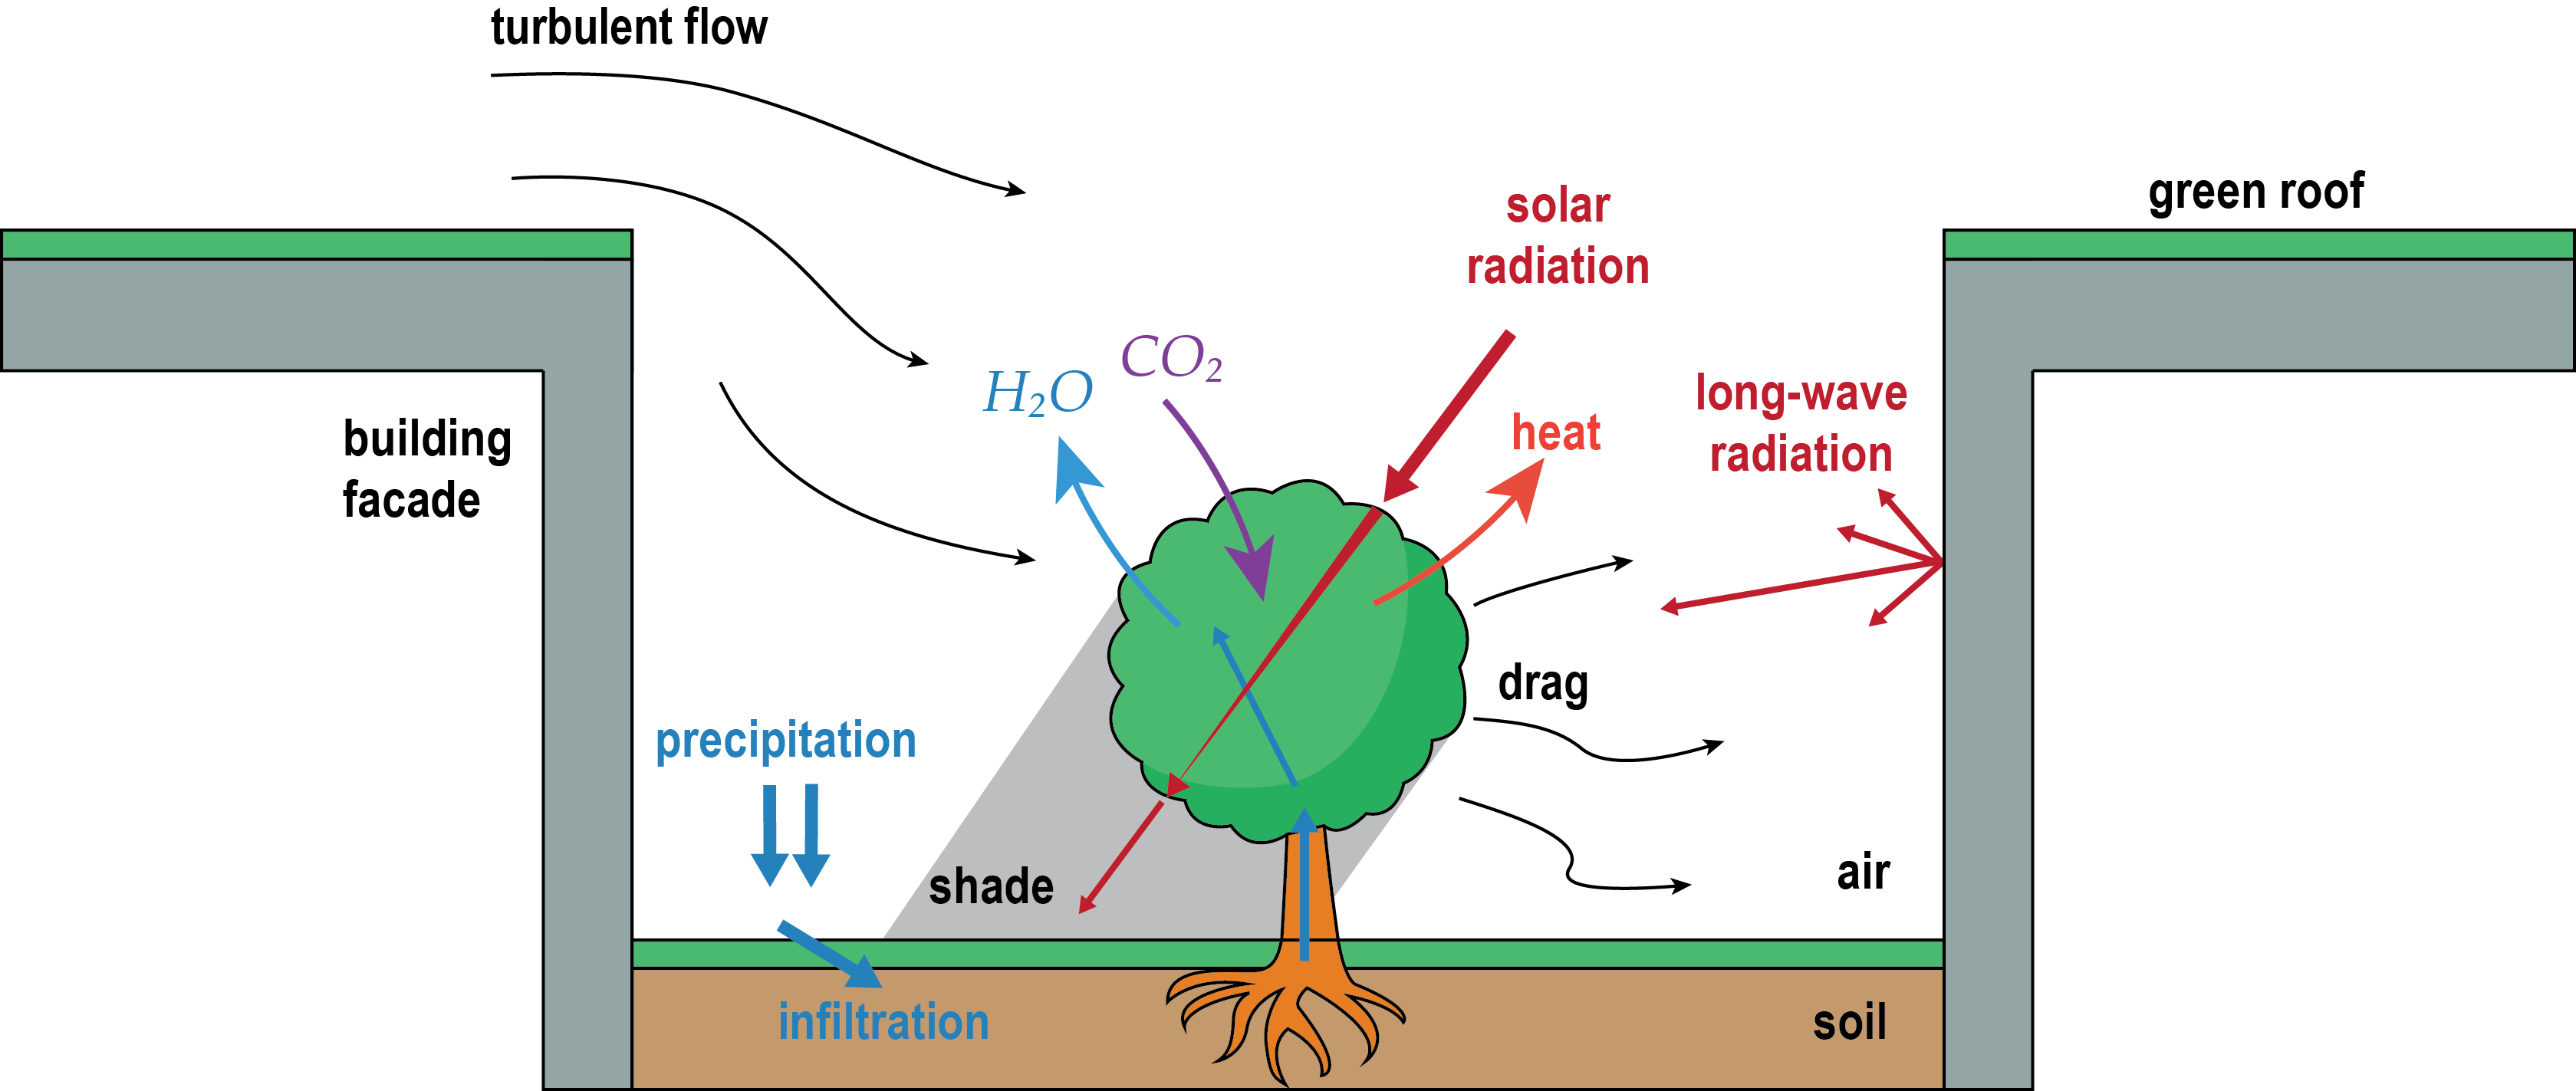
\includegraphics[width=\textwidth]{\figdir/streetcanyon_tree_part5.png}
	\caption{Impact of vegetation on urban microclimate.}
	\label{fig:vegetation_fluxes}
\end{figure}

Thus, there is a need to understand better these complex, coupled, physical processes that contribute to the cooling provided by vegetation. We must better quantify the influence of vegetation on the urban energy balance. Therefore, a multi-domain coupled numerical model is to be developed to elucidate the interactions and the feedback loops of vegetation in an urban context. Furthermore, the water cycle driven by the plant transpiration should be modeled to accurately assess the impact of vegetation on urban microclimate, especially the influence on thermal comfort. Moreover, there is a great need for high-resolution experimental data that can reveal the spatial and temporal variability in the plant responses. \highlight{For example, the leaf temperature is known to be a function of space and the plant transpiration rate is known to vary throughout the day}.

\section{Objective and Methodology}

As vegetation is increasingly being sought after as a natural UHI mitigation strategy, accurate predictions tools need to be available. \highlight{Therefore, the goal of the thesis is:}

\begin{itemize}
	\item \highlight{to assess the impact of vegetation on the microclimate.}
	\begin{itemize}
		\item \textit{airflow}: to better understand how the sheltering provided by small model trees (typically used in wind tunnel experiments) differs from that of natural trees.
		\item \textit{airflow}: to better understand how the seasonal foliar density change affects the sheltering provided by trees.
		\item \textit{hygrothermal}: to quantify the change in urban energy balance due to vegetation.
	\end{itemize}
	\item \highlight{to quantify the natural cooling provided by vegetation.}
		\begin{itemize}
		\item \textit{hygrothermal}: to quantify the difference between transpirative cooling and cooling due to shading by trees.
			\item \textit{hygrothermal}: to quantify the influence of wind speed, air temperature, relative humidity, and solar radiation intensity on the plant cooling potential.					
			\item \textit{hygrothermal}: to quantify the influence of plant properties (i.e., leaf size, stomatal resistance, tree height) and foliage density on the plant cooling potential.			
			\item \textit{hygrothermal}: to better understand the diurnal response of the plant and any spatial and temporal variability in plant condition (i.e., leaf temperature, transpiration rate).	
		\end{itemize}		
	\item \highlight{to understand the influence of water stress on natural cooling.}
		\begin{itemize}
			\item \textit{hygrothermal}: to better understand the feedback loop between soil moisture and plant transpiration.			
			\item \textit{hygrothermal}: to quantify the influence of water availability on the plant cooling potential.
		\end{itemize}
	\item \highlight{to quantify the impact of vegetation on pedestrian thermal comfort.}
		\begin{itemize}
			\item \textit{comfort}: to better understand the governing factor related to vegetation that affect the pedestrian thermal comfort. 				
		\end{itemize}
\end{itemize}



%More specifically, the objective of this thesis is as follows:
%\begin{itemize}
%	\item \textit{airflow}: to better understand how the sheltering provided by small model trees (typically used in wind tunnel experiments) differs from that of natural trees.
%	\item \textit{airflow}: to better understand how the seasonal foliar density change affects the sheltering provided by trees.
%	\item \textit{hygrothermal}: to quantify the change in urban energy balance due to vegetation.
%	\item \textit{hygrothermal}: to quantify the difference between transpirative cooling and cooling due to shading by trees.
%	\item \textit{hygrothermal}: to quantify the influence of wind speed, air temperature, relative humidity, and solar radiation intensity on the plant cooling potential.
%	\item \textit{hygrothermal}: to quantify the influence of plant properties (i.e., leaf size, stomatal resistance, tree height) and foliage density on the plant cooling potential.
%%	\item \textit{hygrothermal}: to better understand the diurnal response of the plant and any spatial and temporal variability in plant condition (i.e., leaf temperature, transpiration rate).
%%	\item \textit{hygrothermal}: to better understand the feedback loop between soil moisture and plant transpiration.
%%	\item \textit{hygrothermal}: to quantify the influence of water availability on the plant cooling potential.
%%	\item \textit{comfort}: to better understand the governing factor related to vegetation that affect the pedestrian thermal comfort. 				
%\end{itemize}

In this thesis, experimental and numerical approaches are combined to assess the impact of vegetation on the microclimate. Experiments in an atmospheric boundary layer (ABL) wind tunnel are opted to understand the impact of vegetation on the airflow and the (near-wake) microclimate, where the small model and natural trees are employed as scaled models. Measurement techniques such as particle image velocimetry (PIV) and drag force measurement are employed to quantify the modification of airflow due to vegetation. Measurement techniques such as infrared thermography and hygrothermal sensor analysis are used to quantify the change in hygrothermal variables of the microclimate. A numerical assessment of the impact of vegetation on urban microclimate is achieved by integrating a vegetation model into a computation fluid dynamics (CFD) model in OpenFOAM. The developed numerical approach simultaneously resolves turbulence modification, radiation balance, heat and mass fluxes, and the sensitivity to soil moisture. The influence of the water availability on the transpiration rate is modeled using a soil-plant-atmosphere continuum (SPAC) model.  Thus, the model is to quantify the cooling potential of vegetation along with its impact on thermal comfort for a pedestrian.

\highlightpara{The present thesis hopes to address the impact of vegetation at a microclimate scale. Therefore, the study aims to prove a better estimation on the efficacy of vegetation as a mitigation strategies for improving human health and thermal comfort in cities. Moreover, the developed numerical model provides the a key element missing in the urban microclimate model in the present research group (i.e., Chair of Building Physics). In future, the detailed model can be enable parametric studies on the role of vegetation in urban environment. Such advanced model will support the design of UHI mitigation strategies by the integration of vegetation in cities. Furthermore, the model can enable to assess the impact of vegetation on wind driven rain. Phenomena such as interception of rain and its impact on pedestrian comfort can now be modeled.}

\section{Outline of the thesis}

This thesis is divided into two parts: i) experimental studies (\cref{ch:paper2,ch:microclimatestudy}), and ii) numerical studies (\cref{ch:parametricstudy,ch:wtcfdcomparison,ch:numericalmethod,ch:impactofvegetation}) of the impact of vegetation on urban microclimate. The thesis is organized as follow:
\begin{itemize}
	\item \textit{Chapter 2}: The chapter addresses state of the art providing an introduction to urban climate, the influence of vegetation at microclimate scale, and typical experimental approaches and numerical approaches for assessing the impact of vegetation. The goal of the chapter is: i) to provide an overview of relevant researches that are present and are employed for quantifying the impact of vegetation on urban microclimate and ii) to justify the scope of the numerical model that is presented in this thesis. 

	\item \textit{Chapter 3}: This chapter is the first part of the experimental studies, where the impact of vegetation on the airflow is investigated. The aim of the study is the understand how the sheltering provided by small model trees differs from that of small natural trees and subsequently quantify the difference with mature trees. The influence of vegetation on the airflow is studied in an atmospheric boundary layer (ABL) wind tunnel using small model and natural trees. In the study, the turbulent airflow behind the trees is studied using particle image velocimetry (PIV) measurement technique and is linked to the drag force measurements using a load cell. The chapter has been published as: Manickathan, L., Defraeye, T., Allegrini, J., Derome, D., \& Carmeliet, J. (2018). ``Comparative study of flow field and drag coefficient of model and small natural trees in a wind tunnel''. \textit{Urban Forestry \& Urban Greening}, 230–239. \url{http://doi.org/10.1016/j.ufug.2018.09.011}.	

	\item \textit{Chapter 4}: This chapter is the second part of the experimental studies, where the impact of vegetation on the microclimate is investigated. The influence of vegetation on the microclimate is studied in the wind tunnel using a small \textit{Buxus sempervirens} plant. In the study, the diurnal dynamics of the plant microclimate of a \textit{Buxus sempervirens} is investigated using various high-resolution non-intrusive imaging techniques. The wake flow field is measured using stereoscopic particle image velocimetry (SPIV), the spatiotemporal leaf temperature history is obtained using infrared thermography, and the plant microstructure metrics such as plant porosity, leaf area density (LAD) is obtained through X-ray tomography. \highlight{This chapter has been submitted as: Manickathan, L., Defraeye, T., Carl, S., Richter, H., Allegrini, J., Derome, D., \& Carmeliet, J. (2018). ``Unveiling dynamic changes in the diurnal microclimate of a Buxus sempervirens with non-intrusive imaging of flow field, leaf temperature, and plant microstructure''. \textit{Submitted to Agricultural and Forest Meteorology}}.

	\item \textit{Chapter 5}: In this chapter the numerical model of assessing the impact of vegetation in urban microclimate is described. The \textit{air} domain solver, the \textit{solid} domain solver, and the \textit{radiation} model is described in detail. Furthermore, the chapter describes the coupling strategy employed to couple these three models with a detailed description of the coupling algorithm. The influence of water availability on transpiration rate is addressed by an advanced stomatal model based on the soil-plant-atmosphere continuum (SPAC) model approach. 

	\item \textit{Chapter 6}: This chapter is the first part of the numerical studies, where the impact of vegetation on the transpirative cooling potential is investigated. The aim of the study is to quantify how much the environmental factors (i.e., wind speed, air temperature, relative humidity, and solar radiation intensity) and tree properties (i.e., leaf size, stomatal resistance, and leaf area density) contribute to the plant cooling performance and the pedestrian comfort. The influence of vegetation on the transpirative cooling is studied using a computational fluid dynamics (CFD) modeling approach, where vegetation is modeled as a porous medium. \highlight{The full-model described in \cref{ch:numericalmethod} is simplified to focus the study on the leaf energy balance and the its influence on the transpirative cooling effect of the atmosphere. Further simplification is performed to enable a rigorous parametric study by only investigating a stand-alone tree at solar noon and the stomatal model is simplified to dependent only on the atmospheric evaporative demand (AED) and solar radiation intensity such that the influence of soil moisture is removed.} The chapter has been published as: Manickathan, L., Defraeye, T., Allegrini, J., Derome, D., \& Carmeliet, J. (2018). ``Parametric study of the influence of environmental factors and tree properties on the transpirative cooling effect of trees''. \textit{Agricultural and Forest Meteorology}, 248, 259–274. \url{http://doi.org/10.1016/j.agrformet.2017.10.014}.

	\item \textit{Chapter 7}: This chapter is focuses on comparing the developed numerical in \cref{ch:parametricstudy} with the microclimate measurements of \cref{ch:microclimatestudy}. The goal of the chapter is to compare and determine the discrepancy of the numerical model in predicting the airflow and the transpiration cooling of vegetation. \highlight{The simplified is used for comparison as the present measurement campaign still lacks the necessary parameters for an accurate calibration of the full-model, such as the plant xylem properties and rhizosphere properties. The present study only focused on the atmospheric changes due to the plant transpiration. In future, a multi-domain measurement campaign consisting of measurements of air domain, soil domain, and plant physiology, can enable the assessment of the full model.} 

	\item \textit{Chapter 8}: This chapter is the second part of the numerical studies, where the impact of vegetation on the urban microclimate is investigated using the numerical model described in \cref{ch:numericalmethod}. The impact of vegetation on the urban microclimate consists of a modification of the turbulent urban airflow, the addition of transpirative cooling in the urban area, and the plant shading provided by the foliage. The influence of these phenomena is investigated together with the impact of pedestrian thermal comfort. 

	\item \textit{Chapter 9}: This chapter provides a conclusion and some of the main finding in the thesis. Furthermore, the chapter provides an overview of the contributions to the research field from the present thesis. Finally, an outlook and possible future research aspects are given.
	
\end{itemize}
